\section{Resultados}
\label{sec:resultados}

A análise identifica uma rede intersetorial quase completa, mas com distribuições de pesos e papéis de atribuição distintos entre atividades. A filtragem reduz o número de ligações e evidencia essas diferenças, com perdas de cobertura desiguais. Os valores apresentados correspondem ao cenário ambiental exploratório descrito na seção~\ref{sec:dados}; não constituem um inventário validado das emissões brasileiras de 2015.

\subsection{Contas ambientais, volume e concentração}

O total atribuído é de 683,70 mil Gg de CO\textsubscript{2} nas duas contas. A diagonal de $F$ reúne 392,92 mil Gg, e as relações entre atividades distintas somam 290,78 mil Gg em $W$. A igualdade entre os totais pela produção e pela demanda decorre da contabilidade; o resultado de interesse é como as mesmas emissões se distribuem entre atividades e contrapartes.

A rede completa tem 67 nós e 4\,290 arestas, com densidade de 97,01\%. As 66 atividades com relações externas estão ligadas entre si nas duas direções e têm graus de entrada e saída iguais a 65. Serviços domésticos (9700) é o único isolado: sua conta permanece na diagonal de $F$. Assim, os graus da rede completa pouco distinguem os perfis, enquanto os pesos mostram diferenças de volume e concentração.

A Figura~\ref{fig:indicadores-resultados} compara essas dimensões para as atividades que compõem a união das seis maiores forças de saída e das seis maiores forças de entrada. Energia (3500) e água, esgoto e resíduos (3680), por exemplo, distribuem volumes externos próximos: 31,32 e 31,23 mil Gg. Entretanto, seus números efetivos de destinos são 20,79 e 9,88. No cenário analisado, volumes semelhantes correspondem a atribuições mais distribuídas em energia e mais concentradas em água e resíduos. Entre os 66 perfis definidos, a mediana é de 11,50 destinos efetivos e 13,93 origens efetivas, abaixo das 65 contrapartes existentes em cada direção.

A Tabela~\ref{tab:contas-energia-construcao} situa energia e construção nas contas completas. Em energia, a produção supera a atribuição pela demanda em 28,39 mil Gg; em construção ocorre o inverso, por 20,56 mil Gg. Os volumes externos mostram como esses saldos se compõem: energia distribui 31,32 mil Gg para outros produtos finais e recebe 2,92 mil Gg de outras origens; construção distribui 2,93 mil Gg e recebe 23,48 mil Gg. A pequena saída externa de construção não indica baixa emissão própria: 35,91 dos seus 38,84 mil Gg pela produção são atribuídos à demanda final da própria atividade e ficam fora de $W$.

\begin{table}[htbp]
\centering
\caption{Contas e volumes intersetoriais de energia e construção.}
\label{tab:contas-energia-construcao}
\small
\begin{tabular}{@{}lrr@{}}
\toprule
Medida & Energia (3500) & Construção (4180) \\
\midrule
Produção, $c$ & 56,62 & 38,84 \\
Demanda, $u$ & 28,23 & 59,40 \\
Atribuição à própria atividade, $F_{ii}$ & 25,30 & 35,91 \\
Saída externa, $s^{\mathrm{out}}$ & 31,32 & 2,93 \\
Entrada externa, $s^{\mathrm{in}}$ & 2,92 & 23,48 \\
Saldo, $u-c$ & $-28,39$ & 20,56 \\
\bottomrule
\end{tabular}
\par\smallskip\begin{minipage}{\textwidth}\footnotesize
Fonte: elaboração própria. Valores em mil Gg de CO\textsubscript{2}, antes do filtro. A diagonal integra $c$ e $u$, mas não as forças externas. Diferenças residuais entre somas de valores exibidos decorrem do arredondamento.
\end{minipage}
\end{table}

\clearpage
\newgeometry{margin=1.5cm}
\begin{landscape}
\begin{figure}[p]
\centering
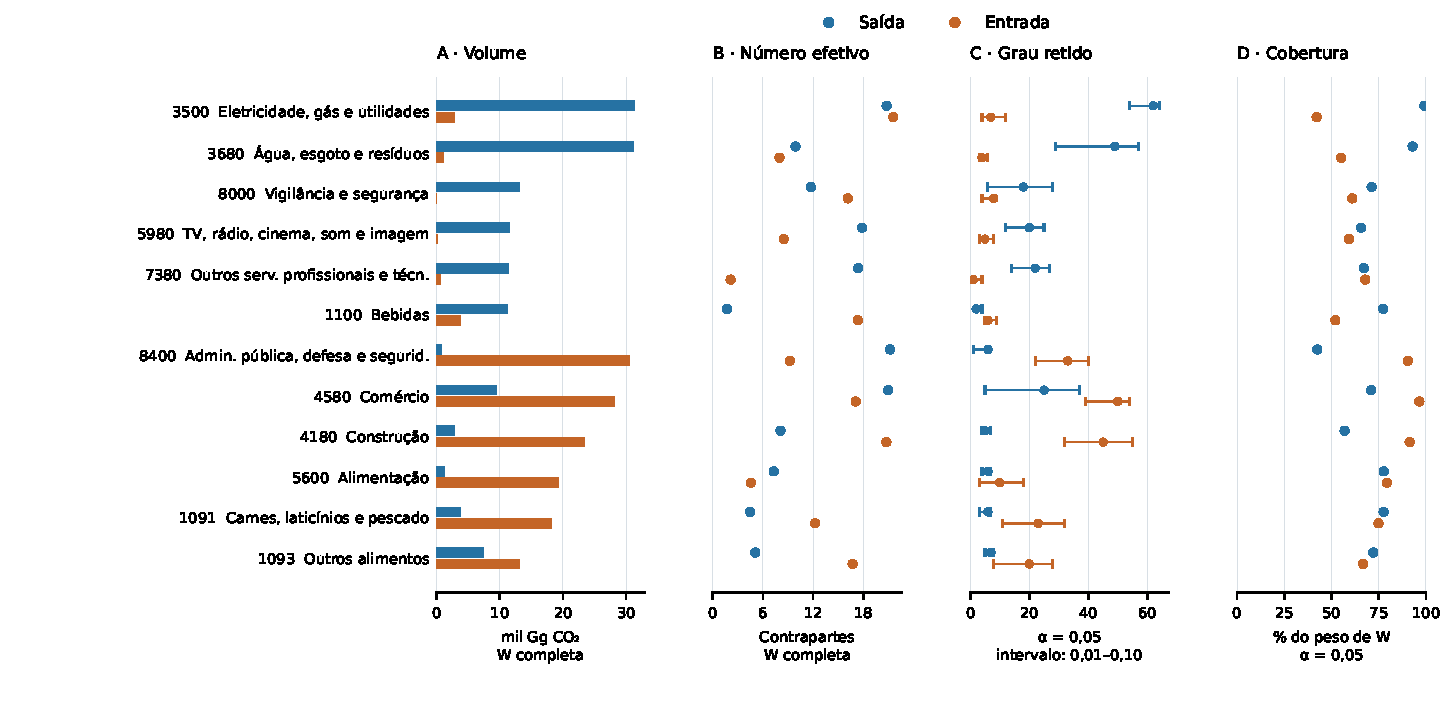
\includegraphics[width=\linewidth,height=0.80\textheight,keepaspectratio]{figuras/indicadores.pdf}
\caption{Volume, concentração, conectividade selecionada e cobertura em atividades de maior volume externo.}
\label{fig:indicadores-resultados}
\begin{minipage}{\linewidth}\footnotesize
Fonte: elaboração própria. Linhas: união das seis maiores forças de saída e das seis maiores forças de entrada de $W$; não representam todas as atividades. Azul: saída; laranja: entrada. Volume e número efetivo são calculados em $W$ completa. Grau e cobertura referem-se a $\alpha=0{,}05$; os intervalos do grau abrangem $\alpha=0{,}01$--$0{,}10$ e não são intervalos de confiança. A diagonal é excluída.
\end{minipage}
\end{figure}
\end{landscape}
\restoregeometry

\subsection{Seleção das relações e limites de cobertura}

O backbone de referência preserva 575 arestas, ou 13,40\% das ligações de $W$, e 70,69\% de seu peso intersetorial (Tabela~\ref{tab:sensibilidade-backbone}). A matriz de adjacência da Figura~\ref{fig:matriz-backbone} mostra essas mesmas relações pela presença e pelo peso. A linha extensa de energia indica muitos destinos retidos; a coluna extensa de construção indica muitas origens retidas. A comparação entre os painéis distingue a existência de uma ligação de seu volume: nem todas as células retidas carregam pesos elevados.

\begin{table}[htbp]
\centering
\caption{Sensibilidade da seleção e da cobertura ao parâmetro do filtro.}
\label{tab:sensibilidade-backbone}
\small
\begin{tabular}{@{}crrrr@{}}
\toprule
$\alpha$ & Arestas & \% das arestas de $W$ & Peso retido & Cobertura (\%) \\
\midrule
0,01 & 338 & 7,88 & 166,88 & 57,39 \\
0,05 & 575 & 13,40 & 205,55 & 70,69 \\
0,10 & 755 & 17,60 & 224,92 & 77,35 \\
\bottomrule
\end{tabular}
\par\smallskip\begin{minipage}{\textwidth}\footnotesize
Fonte: elaboração própria. Peso em mil Gg de CO\textsubscript{2}. Cobertura relativa ao peso de $W$, sem diagonal. Todos os casos mantêm 67 nós, um isolado e um componente fracamente conectado de 66 atividades. O filtro é aplicado à mesma rede completa, com regra OU e sem atualização dos perfis.
\end{minipage}
\end{table}

A cobertura agregada oculta diferenças locais. Em $\alpha=0{,}05$, as medianas entre os perfis definidos são 59,32\% nas saídas e 55,69\% nas entradas; os mínimos são 32,96\% e 33,79\%. Portanto, a preservação de parcela expressiva do peso total não assegura representação igualmente completa de cada atividade e direção.

A sensibilidade também limita a interpretação dos graus. Em relação a $\alpha=0{,}05$, a redução para 0,01 altera os postos de grau de saída em mediana de 11 posições, e os de entrada em sete; a elevação para 0,10 produz mudanças medianas de 4,5 e quatro posições. Os postos consideram empates. A permanência do componente de 66 atividades nos três casos descreve a conectividade agregada, mas não demonstra estabilidade das posições individuais. Mantém-se 0,05 como referência, sem tratá-lo como parâmetro ótimo.

Dos 575 vínculos retidos, 232 passam somente pelo teste de saída na origem, 265 somente pelo de entrada no destino e 78 pelos dois. Nenhum depende da convenção de grau um. Essa composição mostra por que o backbone não equivale a selecionar apenas as maiores emissões absolutas: a relação pode destacar-se em uma ponta e representar parcela pequena da força da outra.

\clearpage
\newgeometry{margin=1.5cm}
\begin{landscape}
\begin{figure}[p]
\centering
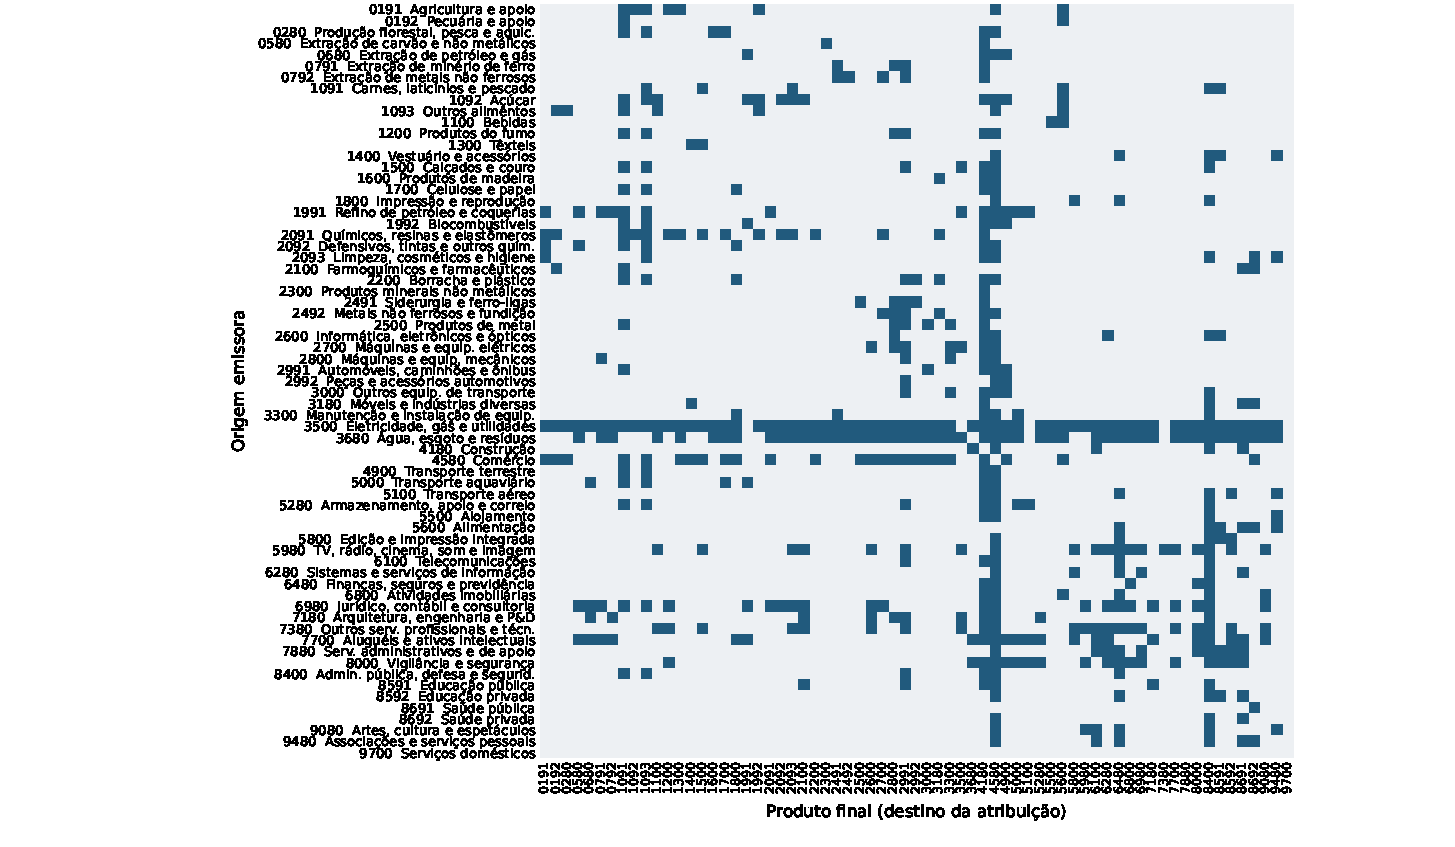
\includegraphics[width=\linewidth,height=0.82\textheight,keepaspectratio]{figuras/matriz_presenca.pdf}
\caption{Matriz de adjacência do backbone com $\alpha=0{,}05$: (a) presença das arestas.}
\label{fig:matriz-backbone}
\begin{minipage}{\linewidth}\footnotesize
Fonte: elaboração própria. Linha: origem emissora; coluna: atividade do produto final. Ordem setorial do IBGE nos dois eixos. Azul identifica as 575 ligações retidas; cinza indica ausência no backbone, inclusive a diagonal. Ausência no backbone não implica valor nulo em $F$ ou $W$. Todas as 67 atividades permanecem nos eixos.
\end{minipage}
\end{figure}
\clearpage
\begin{figure}[p]
\ContinuedFloat
\centering
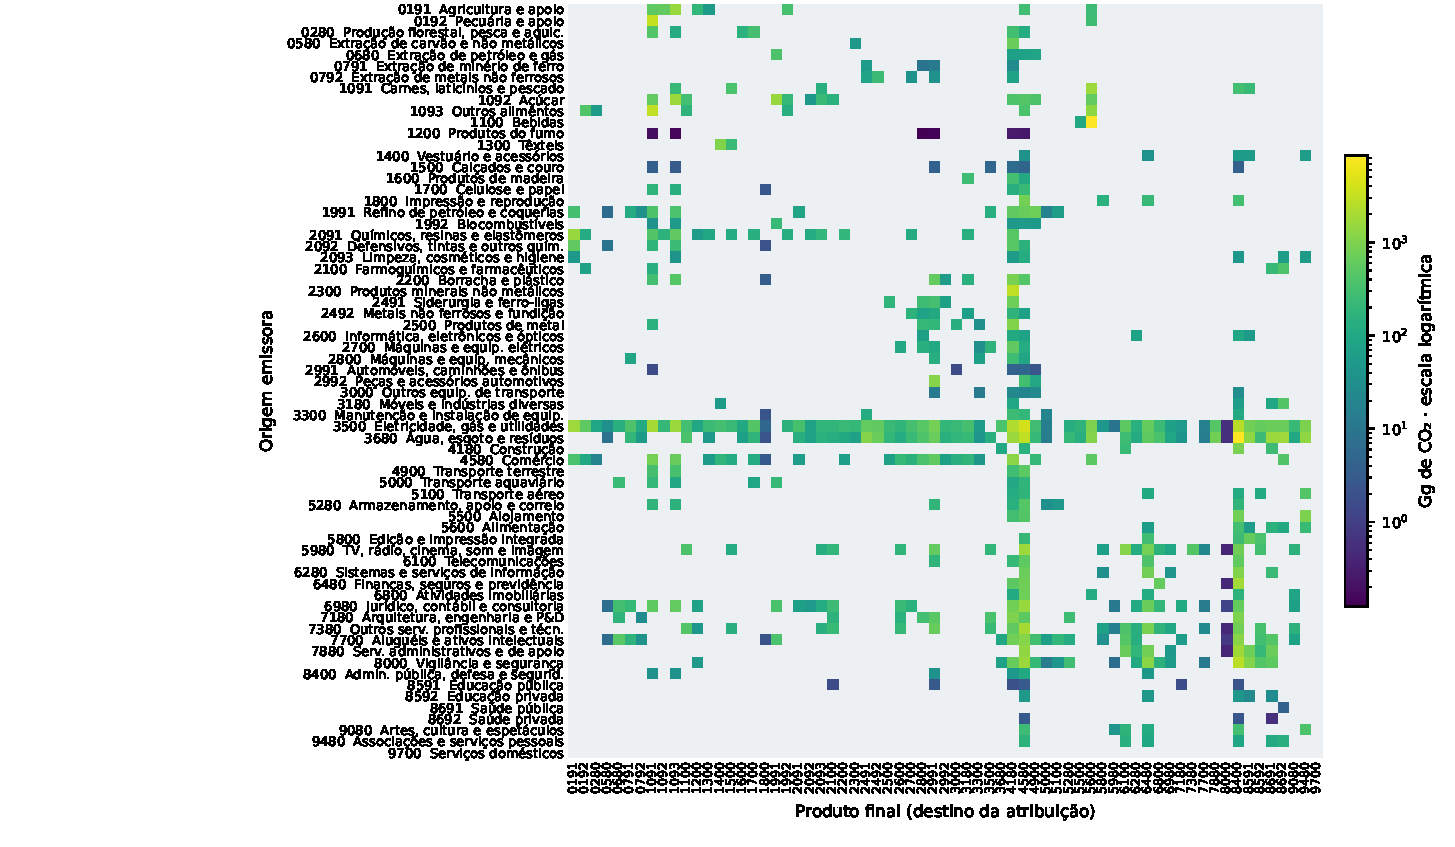
\includegraphics[width=\linewidth,height=0.82\textheight,keepaspectratio]{figuras/matriz_peso.pdf}
\caption{Matriz de adjacência do backbone com $\alpha=0{,}05$: (b) pesos das mesmas arestas.}
\begin{minipage}{\linewidth}\footnotesize
Fonte: elaboração própria. Mesma ordem e mesma seleção do painel (a). A cor representa pesos originais em Gg de CO\textsubscript{2}, em escala logarítmica, sem normalização por linha ou coluna. Cinza identifica células sem aresta retida. A cor mede volume absoluto; a concentração é descrita pelos números efetivos em $W$ completa.
\end{minipage}
\end{figure}
\end{landscape}
\restoregeometry

\subsection{Energia e construção: perspectivas de uma mesma relação}

Energia e construção ilustram dois papéis na atribuição intersetorial: uma origem emissora associada a muitos destinos finais e um destino que reúne emissões de muitas origens. A Figura~\ref{fig:rede-focos} apresenta duas vistas completas do mesmo backbone, com posições idênticas e destaque para as relações de cada atividade. Os 33 nós com $c>u$ ficam à esquerda, os 33 com $u>c$ à direita, e o isolado fica abaixo. Essa organização explicita o saldo já calculado; não resulta de detecção de comunidades. As cores mostram entradas e saídas do destaque, enquanto os motivos de retenção são detalhados na Tabela~\ref{tab:motivos-casos} e nos painéis completos do Anexo~\ref{anexo:paineis}.

\begin{table}[htbp]
\centering
\caption{Motivos de retenção e cobertura nos recortes de energia e construção.}
\label{tab:motivos-casos}
\small
\begin{tabular}{@{}lrrrrr@{}}
\toprule
Recorte & Arestas & Só saída & Só entrada & Ambos & Cobertura (\%) \\
\midrule
Energia: entradas & 7 & 1 & 5 & 1 & 42,1 \\
Energia: saídas & 62 & 0 & 56 & 6 & 99,2 \\
Construção: entradas & 45 & 41 & 0 & 4 & 91,4 \\
Construção: saídas & 5 & 4 & 1 & 0 & 57,0 \\
\bottomrule
\end{tabular}
\par\smallskip\begin{minipage}{\textwidth}\footnotesize
Fonte: elaboração própria. $\alpha=0{,}05$. Saída e entrada nas colunas de motivo identificam o teste na origem e no destino da aresta, independentemente da atividade em destaque. Cobertura: peso retido dividido pela força da mesma atividade e direção em $W$. Os recortes compartilham arestas e não devem ser somados para obter totais da rede.
\end{minipage}
\end{table}

Em energia, 56 das 62 saídas retidas passam somente pelo teste de entrada no destino. A atividade tem participação saliente na composição externa de muitas demandas finais, embora cada destino possa representar parcela pequena das emissões distribuídas pela origem. As outras seis relações passam pelos dois testes. Entre os maiores destinos estão comércio, administração pública, construção e atividades alimentares.

Em construção, 41 das 45 entradas passam somente pelo teste de saída na origem. Construção representa parcela saliente das atribuições externas dessas origens, mesmo quando a contribuição individual é pequena no total recebido pelo destino. As quatro entradas que passam pelos dois testes vêm de produtos de minerais não metálicos, energia, água e resíduos e comércio. A relação energia $\rightarrow$ construção, comum aos dois recortes, pesa aproximadamente 2\,263 Gg: 7,2\% das saídas externas de energia e 9,6\% das entradas externas de construção.

As direções predominantes também apresentam maior cobertura: 99,2\% das saídas de energia e 91,4\% das entradas de construção. Nas direções inversas, ficam fora do backbone 57,9\% das entradas externas de energia e 43,0\% das saídas externas de construção. Assim, os recortes representam bem os volumes predominantes, mas as listas curtas nas outras direções não autorizam desprezar os vínculos omitidos em conjunto. A diferença entre 62 saídas de energia e 45 entradas de construção também não mede concentração: em $W$ completa, os respectivos números efetivos são próximos, ambos de 20,8 contrapartes.

Em conjunto, os resultados mostram relações de pesos desiguais cuja saliência depende da ponta examinada. Forças e números efetivos caracterizam os perfis completos; o backbone identifica contrapartes com cobertura conhecida. O saldo $u-c$ permanece calculado nas contas completas. As arestas descrevem atribuições diretas e indiretas; sua concatenação não representa trajetórias produtivas.

\clearpage
\begin{figure}[p]
\centering
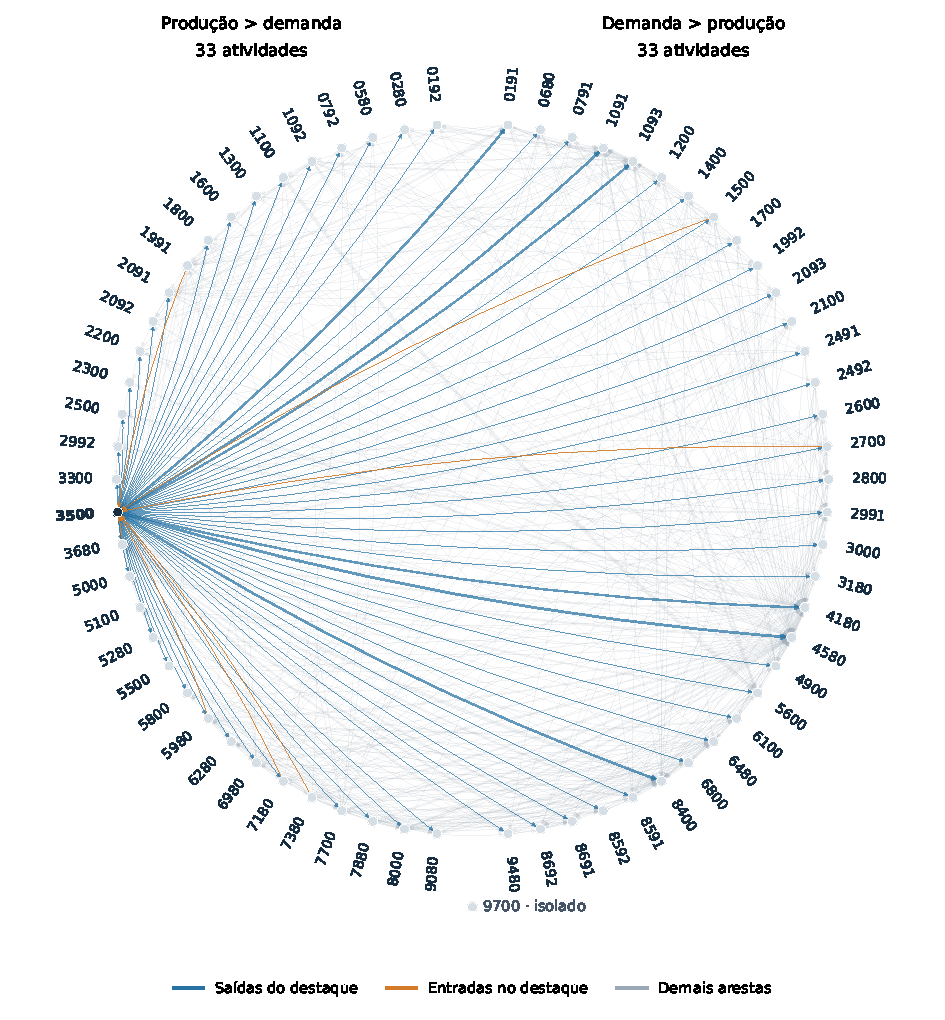
\includegraphics[width=\textwidth,height=0.76\textheight,keepaspectratio]{figuras/rede_foco_3500.pdf}
\caption{Duas perspectivas do mesmo backbone: (a) destaque para energia (3500).}
\label{fig:rede-focos}
\begin{minipage}{\textwidth}\footnotesize
Fonte: elaboração própria. Cada vista mantém 67 nós e 575 arestas em $\alpha=0{,}05$. Azul: saídas do destaque; laranja: entradas; cinza: demais arestas. Energia tem 62 saídas e sete entradas, com cobertura de 99,2\% e 42,1\% do volume externo de cada direção. Área dos nós uniforme; espessura cresce com a raiz quadrada do peso. Posição definida pelo sinal de $u-c$ nas contas completas e pela ordem IBGE em cada lado, não por centralidade ou comunidade.
\end{minipage}
\end{figure}
\clearpage
\begin{figure}[p]
\ContinuedFloat
\centering
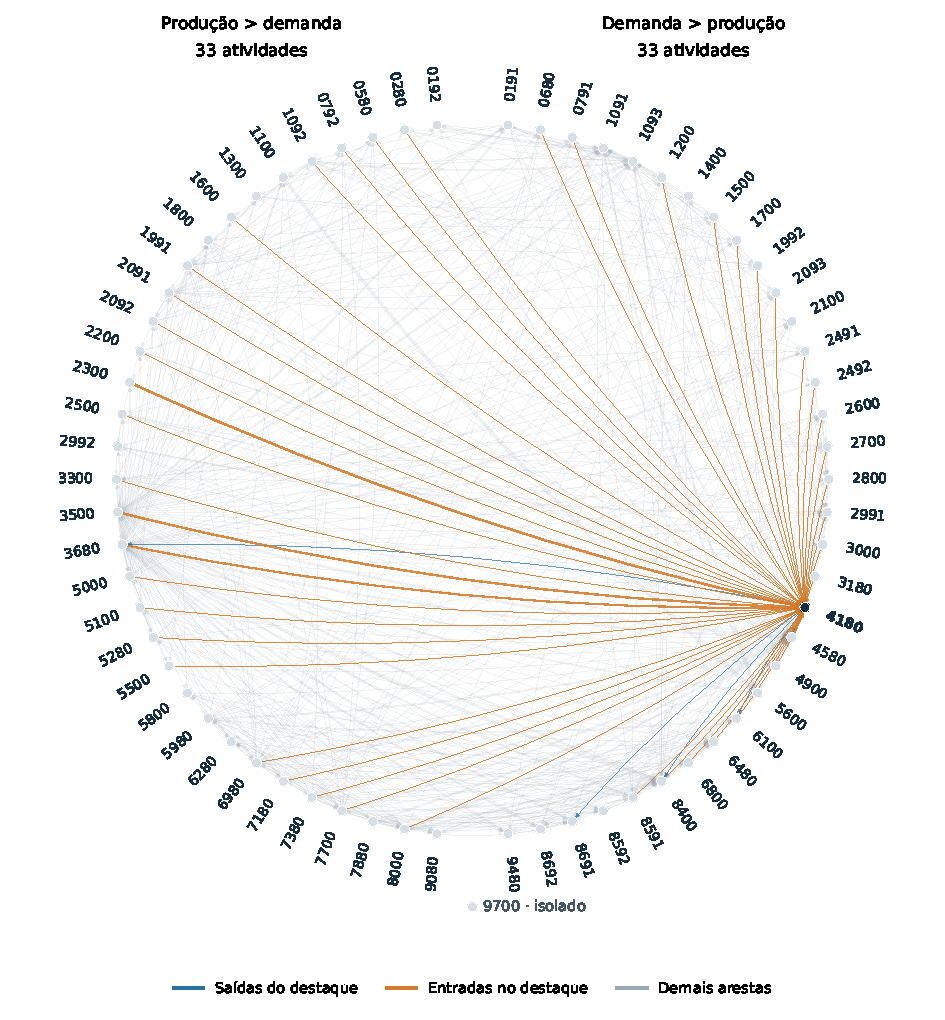
\includegraphics[width=\textwidth,height=0.76\textheight,keepaspectratio]{figuras/rede_foco_4180.pdf}
\caption{Duas perspectivas do mesmo backbone: (b) destaque para construção (4180).}
\begin{minipage}{\textwidth}\footnotesize
Fonte: elaboração própria. Mesmos nós, arestas, posições e escala de espessura do painel (a). Construção tem cinco saídas e 45 entradas, com cobertura de 57,0\% e 91,4\%. Cores representam direção em relação ao destaque, não motivo de retenção. As duas vistas preservam 70,69\% do peso intersetorial de $W$. Cruzamentos e proximidade não representam trajetórias ou distâncias econômicas; relações individuais podem ser consultadas na matriz e nos painéis do anexo.
\end{minipage}
\end{figure}
\clearpage
